% This is the LaTex template file for the Journal "Language Development Research"
% Version: 1.0 (2022)
% Author: Mitja Nikolaus (mitja.nikolaus@posteo.de)
% Compile this file using pdflatex.
% The repository for the source files can be found at
%
%     https://github.com/mitjanikolaus/ldr-template
%

\documentclass{ldr-article}

\addbibresource{main.bib}

% here we can set the page counter to the correct global page counter
\setcounter{page}{1}

% Here we can set the correct volume and issue number for accepted articles
\fancyfoot[C]{\titlepagefontsize Volume X, Issue Y, 31 December 2022}


\title{The title goes here (only the first word has an initial capital) set in the font source sans pro bold 16 point, centered, with line spacing at exactly 18 point. It may span several lines if necessary}


\author{
Andrea N. Other\\
William J. Kramer\\
University of Nowhere, USA
\\\\
Jason Pierce\\
University of Rugby, UK
}



\begin{document}

    \maketitle

    \begin{abstract}
       The simplest way to achieve correct formatting is simply to modify this template but copying and pasting your article into it. However, we give details here for authors who wish to format an existing document manually (including using software other than Word or \LaTeX). The abstract and everything else on the title page (except the title itself) is set in Source Serif Pro regular 10 point, with line spacing exactly 12 point (unlike the main text, which is the same typeface, but 12 point, with line spacing exactly 14 point). The abstract text should be justified at both the left and right edges (this is identical to the body text; there is no additional indentation applied to the abstract). The document should be set to a page size of A4. The entire document should be set up with margins of 4cm at the bottom, 2.5cm at the top, 2.5cm on the left and 2.5cm on the right, with no gutter (0cm). In Word, these settings are accessed via Format > Document > Margins. The header and footer should both be set to 1.50cm (in Word, double click inside the header and enter “1.5cm” in the “Header from Top” and “Header from Bottom” boxes). The abstract should be a maximum of 250 words. After the Abstract, Keywords and License information, the main text should begin on a new page with the heading “Introduction” (or other heading as appropriate). Author notes, acknowledgements etc. should be placed at the end of the paper, after the References but before any Appendices, rather than on the first page. Please avoid changing the orientation of the page as this creates section breaks, which can cause problems regarding the header, footer and page numbers.
    \end{abstract}
    
    \keywords{keywords go here; use 3-5 keywords; semicolons in between; same font as abstract; authors designate their own keywords rather than choosing from a menu.}
    \correspondingauthor{Jason Pierce, Department of Psychology, University of Rugby, Spaceman Park, Rugby, CV21 1XX, UK. Email: Jason.Pierce@Rugby.ac.uk.}
    \orcid{https://orcid.org/0000-1234-5678-9999}
    % for multiple ORCIDs, use \orcids and URLs separated by semicolons, e.g.:
    %\orcids{https://orcid.org/0000-1234-5678-9999;https://orcid.org/0000-5678-1234-9999}
    \citationinfo{Other, A.N., Kramer, W.K., \& Pierce, J. (2022). Article title goes here. \textit{Language Development Research, 2}(1), XX–XX. \url{https://doi.org/10.34xxx/xxxx-xxxx}}



\section{Introduction (Top [Level 1] Headings Use Centered, Bold, Title Case Heading)}

The Introduction should start on a new page. As a fully Open Access journal with no subscription fees or article processing charges, Language Development Research does not employ copyeditors or typesetters: Authors of accepted manuscripts are required to undertake their own copyediting and supply the final typeset and formatted article (i.e., the final author-supplied PDF  is what journal readers will download). The guidelines set out here have been designed to yield a finished article that has a distinctive look and feel, and can be achieved relatively easily with any of the packages that are commonly used by academic authors. Word users should not have to edit any of these settings manually. Rather use the “Styles” pane on the “Home” tab to assign pre-defined styles to portions of you text (e.g., “LDR Article Main Title” to your title; “Normal, LDR Normal, Body, Abstract” to your body text; “Heading 1, LDR Heading 1” to Level 1 headings etc.). Ticking the “Show styles guides” box allows you to see at a glance the styles assigned to each portion of text.

The body text is set in Source Serif Pro regular 12 point, with line spacing exactly 14 points (in Word, highlight the entire body text, then choose Format > Paragraph, then under Spacing set “Line Spacing:” to “Exactly” and “At:” to “14 pt”). The OpenType fonts Source Sans Pro and Source Serif Pro are embedded in the .docx template, and so should not normally need to be manually installed. However, if necessary, they can be downloaded from \url{https://github.com/adobe-fonts/source-sans-pro} and \url{https://github.com/adobe-fonts/source-serif-pro} (consult your operating system documentation for how to install fonts). The body text should be justified at both the left and right edges, and automatic hyphenation turned on (in Word, choose Tools > Hyphenation and tick the box “Automatically hyphenate document”, leaving “Limit consecutive hyphens” set to “No limit”). New paragraphs should not be marked with an indentation (except when required for Level 4 and Level 5 headings), but with a blank line of exactly 14 points (this is the default in Word, but can be set manually: highlight the entire body text and choose Format > Paragraph > Indents and Spacing and untick “Don’t add a space between paragraphs of the same style”, also unticking “Snap to grid when document grid is defined”). However, in order to ensure blank lines between authors from the same institution, the box “Don’t add a space between paragraphs of the same style” should be ticked when the authors are being formatted. In order to ensure consistency between documents produced in different packages (Word, LaTeX etc.), users should disable Widow/Orphan control. In Word, highlight the entire document and choose Format > Paragraph > Line and Page Breaks and ensure none of the boxes under “Pagination” are ticked.

Please do not insert two spaces after a period. This (now outdated) convention was only ever meant to apply to draft manuscripts, not typeset, published documents (which is what Language Development Research requires authors to create upon acceptance).

\section{Study 1 (Top [Level 1] Headings Use Centered, Bold, Title Case Heading)}

After top level (Level 1) headings, the text begins with a new paragraph. In general, the APA 7th edition guidelines for levels of heading should be used (\url{https://apastyle.apa.org/style-grammar-guidelines/paper-format/headings}). The only exceptions are (1) the Abstract and Keywords sections which are always set in bold, flush left, initial capitals, followed by a colon, as shown above and (2) the Introduction, which DOES have its own (top level) heading. Note that (unlike in previous APA formats), all headings have Title Case Heading – i.e., the initial letter of all major words are in upper case (short [i.e., three letters or fewer] conjunctions, short prepositions, and all articles are considered minor words). Headings should not be numbered or lettered.

\begin{figure}[htb]
\center{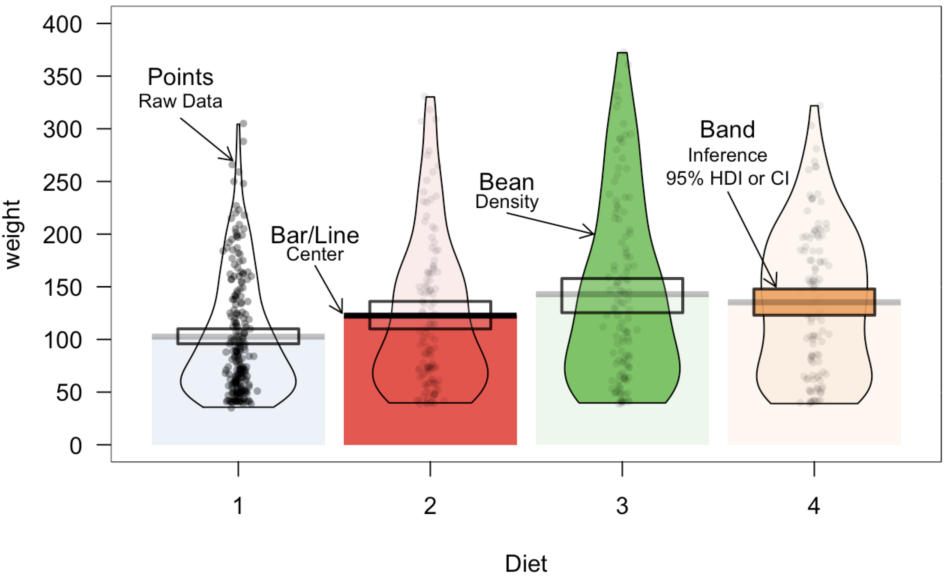
\includegraphics[width=\textwidth]{figures/example_figure.pdf}}
\caption{\label{fig:example_figure} The four elements of a pirate plot (reproduced from Phillips, 2018)}
\end{figure}

Figures and tables should be inserted directly into the main body of the manuscript, not on separate pages at the end, and should be referred to in the text (see Figure \ref{fig:example_figure}). Word users may wish to use the Officer R package which enables figures and tables created in R to be directly inserted into Word documents. Both figures and tables, as well as their captions, should use the default font (Source Serif Pro 12pt) as much as possible: The majority of packages used for creating figures and tables allow custom fonts to be used. However, when this is not the case, other fonts are permitted. Other font sizes may be used if this is required for clarity, or in order for the figure/table to fit within the margins of the document.  Captions should be left justified (rather than left and right justified) in order to avoid excessive white space in between words. Authors should use the “Alt-text” feature of their chosen software (In Word, right click and choose “Edit Alt Text…”) to provide a text description of the figure (since the journal hosting is publicly funded, this constitutes a legal accessibility requirement). 

Figures/tables should be formatted to span the same width as the body text (see Figure \ref{fig:example_figure} and Table \ref{tab:example_table}); they should not be narrower unless this is unavoidable for legibility reasons and must never extend into the margins of the document. Very large figures/tables may be rotated 90 degrees (counter-clockwise) and placed on a separate page (though still in the main body of the manuscript, not at the end).

Figure captions should be placed below the relevant figure and formatted as per the example above; i.e., “Figure X” in bold, and the caption in bold italics. For Word users, one way to keep the figure and its caption together is to insert a table with a single column and two rows, placing the figure in the top row and the caption in the row below it (ensuring the table borders are white, and so invisible).

\begin{table}[htb]
    \caption{Mean scores (and standard deviations) for adults and children in the Experimental and Control groups\label{tab:example_table}}
    \centering
    \begin{tabular}{llll}
        Age Group   & Training Group & Mean & SD \\
        \hline
        Children    & Experimental Group & 55.81 & 23.05 \\
                    & Control Group & 35.25 & 22.28 \\
        \hline
        Adults      & Experimental Group & 67.45 & 15.84 \\
                    & Control Group & 40.41 & 15.04 \\
    \end{tabular}
\end{table}

Figures illustrating data should show not just means for each group, but some clearly labelled measure of distribution (e.g., 95 confidence/credibility intervals) and, ideally, the raw data (e.g., the R PiratePlot package, which was used to create Figure \ref{fig:example_figure}).

Table captions should be placed above the relevant table and formatted as per the example below; i.e, i.e., “Table X” in bold, and the title in bold italics. As for figures, Word users can ensure that the caption moves with the table by including the caption as a row in the table itself (using “merge cells” if necessary). Tables should, in general, follow APA 7th Edition formatting guidelines (e.g., horizontal lines only, no shading, minimal use of bold/italics for column headings), though clarity should always be the overriding concern.

\subsection{Method: Level 2 Headings Use Flush Left, Bold, Title Case Heading}
After Level 2 Headings, the text begins as a new paragraph. Lorem ipsum dolor sit amet, consectetur adipiscing elit. Nunc non aliquet libero. Nam tincidunt justo at ipsum auctor, eu elementum libero faucibus. Praesent in leo ut leo consectetur posuere vitae et libero. Donec elementum felis vulputate, pulvinar enim id, mollis elit. Pellentesque pretium neque vel lorem sagittis egestas. Suspendisse potenti. 

\subsubsection{Participants: Level 3 Headings Use Flush Left, Bold Italic, Title Case Heading}

After Level 3 headings, the text begins as a new paragraph. Ut in felis facilisis, rhoncus orci eget, rutrum mi. Aenean convallis dolor erat. Mauris et aliquet nibh. Mauris eu eleifend purus. Morbi eu interdum sapien, id porta tellus. Etiam placerat ipsum odio, eget semper nisi finibus at. Vestibulum tristique, tellus at venenatis varius, erat lorem consequat sapien, at semper metus dolor non felis. 

\paragraph{Children: Level 4 Headings Use Indented, Bold, Title Case, Ending with a Period.}
After Level 4 headings, the text begins on the same line and continues as a regular paragraph.

\subparagraph{Experimental Group: Level 5 Headings Use Indented, Bold Italic, Title Case, Ending with a Period}
After Level 5 headings, the text begins on the same line and continues as a regular paragraph.

\subparagraph{Control Group}
After Level 5 headings, the text begins on the same line and continues as a regular paragraph.

\subsubsection{Design and Procedure (Level 3 Heading)}
Ut morbi tellus nisi, rutrum sed vestibulum a, luctus sed urna. Morbi ornare ex massa, sit amet finibus dolor tincidunt eget. In efficitur elit at eros consequat, ac varius sapien semper. Curabitur eleifend tincidunt ligula. Suspendisse potenti. Donec blandit aliquam vestibulum. Mauris eu luctus nisi. Pellentesque varius dapibus est non porta. Donec sit amet pulvinar nulla.

\subsection{Results (Level 2 Heading)}

Nulla facilisi. Nunc eu mattis felis. Vestibulum ante ipsum primis in faucibus orci luctus et ultrices posuere cubilia Curae; Nullam vel ornare ligula. Duis aliquam leo suscipit urna dapibus lacinia. Aenean eu condimentum justo. Nam eleifend felis ut pharetra luctus. 


\subsection{Discussion (Level 2 Heading)}

\section{Study 2 (Level 1 Heading)}

Mauris auctor auctor ligula et rhoncus. Quisque tellus erat, laoreet ac nibh pulvinar, scelerisque feugiat orci. Suspendisse fringilla sed odio non ornare. Vestibulum vitae iaculis sapien. 

\section{General Discussion (Level 1 Heading)}

Praesent at quam ac lorem scelerisque consectetur consequat in tortor. Aenean pulvinar felis lorem, nec sollicitudin est laoreet a. Fusce sit amet sem eu dolor iaculis scelerisque in in arcu.


\nocite{other2019references,kramer2019why,phillips2018yarrr}

\printbibliography


\section{Data, Code and Materials Availability Statement}
In order to proceed to peer review, submitted articles must include a “Data, code and materials availability statement” which includes links to permanent repositories (with Digital Object Identifiers [DOIs] wherever possible) and details of any exemptions agreed. Authors applying for an exemption should submit their article in the usual way, setting out the reason for their application in the “Comments to Editor” box. Exemptions are granted by the Editor, but for complex cases, the Editor may first discuss the proposed exemption with the Editorial Board. Generally, exemptions to data/code/materials sharing will be granted only where it is impossible or infeasible (e.g., prohibitively expensive) due to insurmountable concerns regarding participant confidentiality or restrictions imposed by an ethics committee, institutional review board, funder, or local rules, regulations or laws

If data/code/materials are already publicly available (e.g., CHILDES corpora, many government datasets), with or without a free application process, researchers should provide the relevant permanent links in their “Data, code and materials availability statement”, and do not need to duplicate the material in their own project repository.

 “As open as possible”: Where full sharing is not possible for one of the reasons above, authors should, when applying for the relevant exemption, set out the steps that they will take to make the data/code/materials as open as possible. One option, for example, is to deposit data with a service such as the UK Data Service which has separate categories for (in addition to Open Data) Safeguarded and Controlled Data, and separate application procedures for each. Any such arrangements must be documented in the paper’s “Data, code and materials availability statement”. The principle of “as open as possible” will also apply when the journal considers exemption requests. For example, if an exemption is granted on the basis of confidential data, authors will still be required (unless separate exemptions are granted) to share materials and analysis code. Where one or more exemption is agreed, the authors must ensure that it would be possible for a third party to verify the veracity of their findings should a question arise, and their “Data, code and materials availability statement” should clearly articulate a plan for making the necessary data/code/materials available.

Following the principle of “as open as possible”, data should be shared at as raw a level as possible without compromising participant anonymity. For example, if authors created new audio or video recordings which they then transcribed and coded, they should share the transcriptions, and the coded data (unless relevant exemptions have been granted), but not the actual recordings (unless they have explicit permission from the participants to do so). In normal circumstances, data aggregated at the participant or item level, rather than individual participant-by-participant and trial-by-trial data, would not meet the journal’s requirements. 

Unless an exemption has been granted, authors are required to share all the analysis code that would be required for a colleague to reproduce all summaries (e.g., figures/tables) and analyses reported in the paper. Code must be included not just for the final analyses, but for any preprocessing/data-cleaning steps. Note that many point-and-click statistics packages (including SPSS and Stata) can additionally generate analysis code (syntax) files for sharing. If authors used a package (e.g., JASP) or website that does not generate shareable code, they should instead share a screen grab video of the analysis, or a document setting out point-by-point the steps taken. In either case, authors must double check that following the video/document yields the same output as the analysis reported in the paper.

Unless an exemption has been granted, authors are required to share all materials that would be required for a colleague to replicate the study (e.g, questionnaires, ratings-scales, pictures, animations or videos, audio recordings, visually-presented sentences etc.). In particular, if the authors used software such as PsychoPy, jsPsych, PEBL, etc. they should be sure to share the code needed to run the experiment and, for online platforms such as Gorilla, links to the online experiment.

The journal itself does not offer hosting for data/code/materials. Instead, authors should use websites such as the Open Science Framework (\url{https://www.osf.org/}) Figshare (\url{https://figshare.com/}), TalkBank (\url{https://talkbank.org}), Databrary (\url{https://nyu.databrary.org/}) or Github (\url{https://github.com/}), providing the relevant links in their “Data, code and materials availability statement”. Other sites may be used, but authors must use permanent repositories, not personal/institutional websites, or folders on platforms such as Dropbox, Google Drives etc. Language Development Research is the official journal of the Talkbank system \url{https://talkbank.org/}, and, as such, the journal requests that any new corpora reported in LDR papers be posted to the relevant TalkBank site: CHILDES (Child Language Data Exchange System), PhonBank, Homebank, or one of the dedicated Multilingualism, Clinical or Adult Conversation banks.

\section{Ethics statement (Level 1 Heading) – Mandatory for Empirical Articles}
Ethics approval was obtained from the ethics committee of the University of Nowhere. All participants gave informed written consent before taking part in the study.

\section{Authorship and Contributorship Statement}
ANO conceived of the study, designed the study and wrote the first draft of the manuscript. WJK contributed to the design of the study, collected the data, and revised the manuscript. JP analysed the data and revised the manuscript. All authors approved the final version of the manuscript and agree to be accountable for all aspects of the work in ensuring that questions related to the accuracy or integrity of any part of the work are appropriately investigated and resolved. For guidance, please see \url{http://www.icmje.org/recommendations/browse/roles-and-responsibilities/defining-the-role-of-authors-and-contributors.html}.

\section{Declaration of conflict of interests}
A declaration of conflict of interests section is mandatory only if a conflict of interest exists. This section should be deleted if no conflict of interests exists.

\section{Acknowledgements, author notes etc. (Level 1 Heading)}
Integer id tincidunt sem. Aenean urna est, hendrerit at imperdiet sit amet, faucibus non elit. Duis ultrices mauris quis lobortis dapibus. Pellentesque id sollicitudin turpis. Donec eleifend odio gravida sem efficitur viverra. Etiam vel turpis quis nulla accumsan posuere. Etiam dignissim aliquet mattis.


\clearpage
\appendix

\section{Appendices etc. (Level 1 Heading)}

Integer id tincidunt sem. Aenean urna est, hendrerit at imperdiet sit amet, faucibus non elit. Duis ultrices mauris quis lobortis dapibus. Pellentesque id sollicitudin turpis.



\section{License}
Language Development Research (ISSN 2771-7976) is published by TalkBank and the Carnegie Mellon University Library Publishing Service. Copyright © 2022 The Author(s). This work is distributed under the terms of the Creative Commons Attribution Noncommercial 4.0 International license (\url{https://creativecommons.org/licenses/by-nc/4.0/}), which permits any use, reproduction and distribution of the work for noncommercial purposes without further permission provided the original work is attributed as specified under the terms available via the above link to the Creative Commons website.

 

\end{document}
